
\section{Vine as a New Form of Expression}
\label{sec:new-vine-old-bottle}

\vspace{-2mm}
\begin{figure}[!htb]
\centering
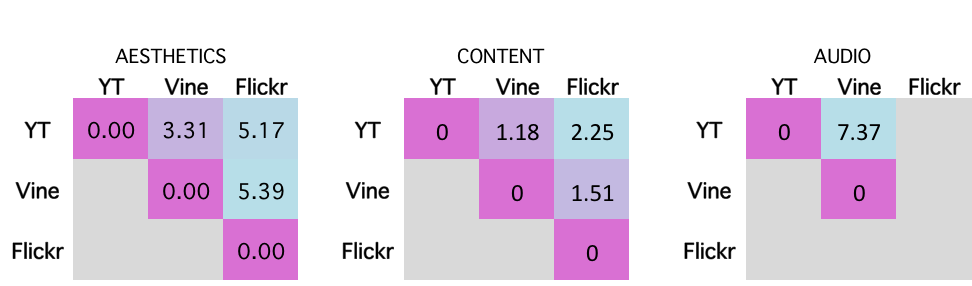
\includegraphics[width=\columnwidth]{plots/comparison/table}
\caption{\textsl{ Aggregated symmetric KL Divergences between platforms over all features for different feature groups.}}
	\label{fig:comparisontable}
	\vspace{-2mm}

\end{figure}


%As pointed out  by previous work \cite{redi20146}, micro-videos have been often called a ``new form of expression'' that goes beyond the traditional video medium.  Vine constraints (short length, limited editing tools) offer an unprecedented number of possibilities for creative visual artists. Tech journalists \footnote{\small \url{https://www.scientificamerican.com/article/why-micro-movies-so-popular-today/}} have indeed theorised that micro-videos cannot be even categorised as videos: their goal is to capture a single moment, thus making them ideally close to the photographic medium, or  \emph{``neither photo nor video but something in between, with artistic merits all its own''}. 

To understand the role of Vine and the different features of its videos,  we begin by comparing Vine with Flickr and YouTube, and test the conjecture that Vine is a new form of expression that is different from both images and videos~\cite{pogue13}.  We focus on items which have engaged large numbers of users, and compare our dataset of popular Vines (POP12K) with datasets of popular images from Flickr and videos on YouTube.  Specifically, we compare the features of POP12K vines with the corresponding features from a sample of 1000 popular\footnote{i.e., with high  ``interestingness'' rating -- https://www.flickr.com/explore/interesting rating}  images from the MIR-Flickr dataset~\cite{huiskes08}, and 419 viral YouTube videos~\cite{Jiang:2014:VVS:2578726.2578754}. To compare all the datasets as images, we sample the videos at the rate of 1 image per second producing several still images, whose parameters we study. We compare these datasets along several dimensions as below.

\subsection{Visual quality comparison} 
We describe each Flickr image, YouTube video or Vine micro video with the 18 computational aesthetics features from \S\ref{sec:features} (Table~\ref{tab:Features_table}). Then, for each feature and dataset, we compute the  marginal probability distribution of the feature on the dataset. %These distributions capture the platforms' dominant visual aesthetics patterns (e.g. what are the common brightness values in YouTube videos? Or the distribution of Colorfulness in Vine?). 
We measure the distance of the marginal distributions of a feature across platforms  (e.g. Rule of Thirds in Flickr vs.\ rule of Thirds in Vine) using symmetric Kullback-Liebler (K-L) divergence. For a given pair of platforms, the average of the K-L divergence values across all features tells us how far apart the two platforms are in the aesthetics feature space. As expected, we find (Fig.~\ref{fig:comparisontable})  that Vine videos show different aesthetic behaviour from both Flickr and YouTube, although they are more stylistically similar to YouTube videos than Flickr images.

%To obtain a description of the visual aesthetics trends for each medium, we aggregate the computed features at a platform-level. To do so, for each dataset, we compute the feature marginal probability distribution. This reflects the platforms' dominant visual aesthetics patterns (e.g. what are the common brightness values in YouTube videos? Or the distribution of Colorfulness in Vine?). To compare distributions across platforms (e.g. Rule of Thirds in Flickr VS Rule of Thirds in Vine), we then use symmetric Kullback-Lieber (KL) divergence, which reflects the distance of 2 probability distributions. The average of such KL divergence values  tells us how far platforms are in the visual aesthetics feature space. We report the results of this analysis in Fig.~\ref{fig:comparisontable}: as expected, Vine videos show different visual aesthetic behaviour from both Flickr and Youtube, although more stylistically similar to long videos. 

\begin{figure}[!htb]
\centering
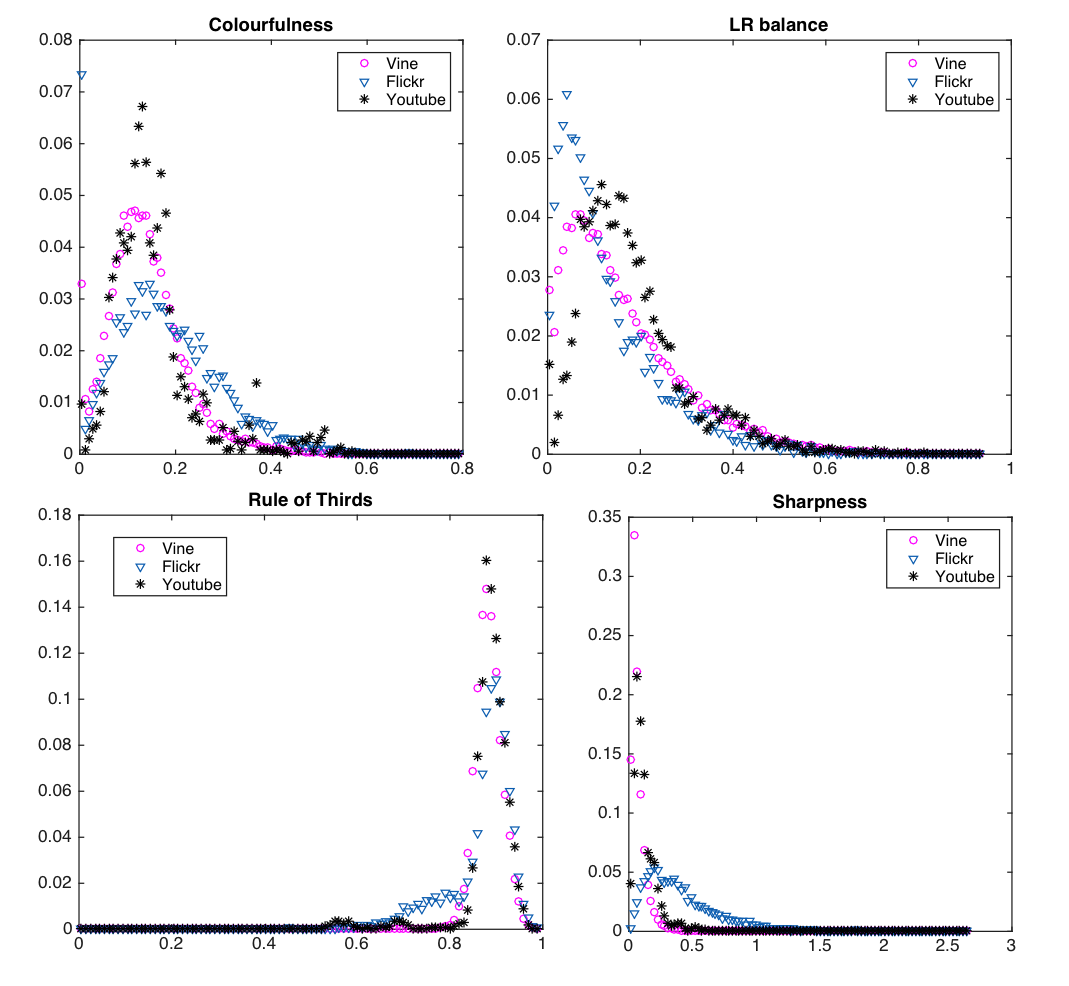
\includegraphics[width=\columnwidth]{plots/comparison/aesthetics}
\caption{\textsl{ Distributions of the most diverging aesthetic features across platforms.}}
\label{fig:comparison_aesthetics}
\end{figure}


To understand why Vine is so different, we look at the features with the highest KL divergence across platforms. We notice that, in practice, Flickr aesthetic features reflect the behaviour of a ``professional'' medium. At the other end of the spectrum, micro videos show patterns of less professional use, typical  of the  user-generated, mobile-first Vine content. Youtube lies in the middle. More specifically, we notice the following (See Fig. \ref{fig:comparison_aesthetics}). (1) \emph{Colorfulness:}  Flickr photos tend to have a higher color diversity, while Vine and Youtube tend to have less saturated colors. (2) \emph{Exposure:}  Flickr pictures tend to have a good balance between Left and Right  pixel intensities, typical of high quality images; unlike Flickr, Youtube and Vine videos show unbalanced exposure. (3) ) \emph{Rule of Thirds:}  Some Flickr pictures tend to deviate from the standard rule of thirds, as it occasionally happens for professional, artistic pictures~\cite{freeman2007photographer}. On the other hand, the moving images of Vine and Youtube tend to stick to the Rule of Thirds heuristic. (4) \emph{Sharpness} is probably one of the most important properties of high quality visual content. Due to its mobile-based nature, Vine videos tend to have almost no sharp pixels, while the professionality of Flickr photographers is clearly exposed by the higher percentage of sharp pixels.

%%%%%%%%%%%%%%%%%%%% TEMPORARILY COMMENTED OUT  
%%\mr{this is raw from the insight sec, still need to do a pass on it, just tied it to the rest in the firs sentence}
%To further explore the relation between Vine and aesthetics, we compare the aesthetic features of frames sampled from both high engagement micro videos and low engagement videos, with highly aesthetic images (rated $>$ 6 on a scale from 0 to 7), taken from the dataset sourced from photo.net \cite{datta2008algorithmic}. %These images were rated for aesthetic appeal for the research involved and these ratings are also used while selecting the images for our comparison. We only choose images with median ratings of 6 \ns{Can you see if we get the same result for median ratings of a=4+? Choosing the lowest value of a makes the case stronger, and helps understand exactly how bad vine videos are} or above on aesthetic scale of 0 to 7.  
%Table~\ref{aesthetic_table} shows the comparison of means and medians of several of these aesthetic features compared to the highly aesthetic dataset. We can observe that popular and unpopular vines show similar values on most parameters considered, yet the scores are way below the values for most  aesthetically pleasing images from photo.net. %Thus, we conclude that whiles aesthetics in micro videos matter, we would not call them aesthetically pleasing. 
%
%\begin{table}
%\caption{List of Aesthetic parameters computed for highly rated aesthetic images, Popular videos and unpopular videos. Most parameters have no bias towards either popular or unpopular videos}
%
%\resizebox{\linewidth}{!}{%
%\begin{tabular}{|l|*{11}{c|}}
%  \hline
%   Parameter & \multicolumn{2}{|c|}{Aesthetic Images}  &  \multicolumn{2}{|c|}{Popular Vines} & \multicolumn{2}{|c|}{Unpopular Vines} \\ \hline
%   \_ & Mean&Median&Mean&Median&Mean&Median\\ \hline
%   \ Color Contrast & 51.05 & 30.22 & 29.88 &16.43 & 20.23  & 8.83  \\ \hline
%   \ Intensity Balance & 0.11 & 0.08 & 0.16 & 0.13 & 0.17 & 0.14 \\ \hline
%   \ Luo Simplicity & 0.009 & 0.005 & 0.013 & 0.012 & 0.015  & 0.014  \\ \hline
%   \ Sharp pixel proportion & 0.103 & 0.098 & 0.090 & 0.085 & 0.089  & 0.081  \\ \hline
%   \ Image Saturation & 0.943 & 0.974 & 0.672 & 0.678 & 0.615  & 0.646  \\ \hline
%   \ Avg. Brightness & 0.148 & 0.141 & 0.137 & 0.130 & 0.139  & 0.124  \\ \hline
%   \ Rule of Thirds & 0.879 & 0.899 & 0.883 & 0.883 & 0.878  &0.882  \\ \hline
%   \ ROI Proportion & 0.316 & 0.089 & 0.175 & 0.112 & 0.165  & 0.110  \\ \hline
%\end{tabular}}
%\label{aesthetic_table}
%\end{table}
%%%%%%%%%%%%%%%%%%%%%%%%%%%%%%%%%%%%%

\subsection{Audio Channel Comparison.} 

The audio channel is as important as the visual channel for long viral videos\footnote{http://thenextweb.com/socialmedia/2015/03/20/set-the-tone-the-importance-of-sound-in-viral-videos/}. We want to understand here the role of audio in  Vine videos. For Youtube and Vine, we extract the audio features in \S\ref{sec:features}. Given the continuous nature of these features, we follow the same procedure used for  aesthetic feature analysis (per-feature symmetric KL divergence). In Fig. \ref{fig:comparisontable}, we see that in the audio space such media are far apart. This is due to the fact that, while the audio tracks of Youtube Videos are very diverse, and therefore follow almost-uniform distributions across different feature ranges, all audio tracks in Vine videos tend to have very similar patterns. In Vine, audio is mainly a weak complement to the visual counterpart: Vine videos can be fully consumed and understood without the audio channel, and they are often played in the mute mode. As a matter of fact, Vine videos tend to have few rythmical changes (low \emph{Onset Rate}) and low \emph{Roughness}. Also, overall, due to their less curated audios, Vine videos tend to be louder than Youtube videos (high \emph{Energy}), as shown in Fig. \ref{fig:comparison_audio}.
\begin{figure}[!htb]
\centering
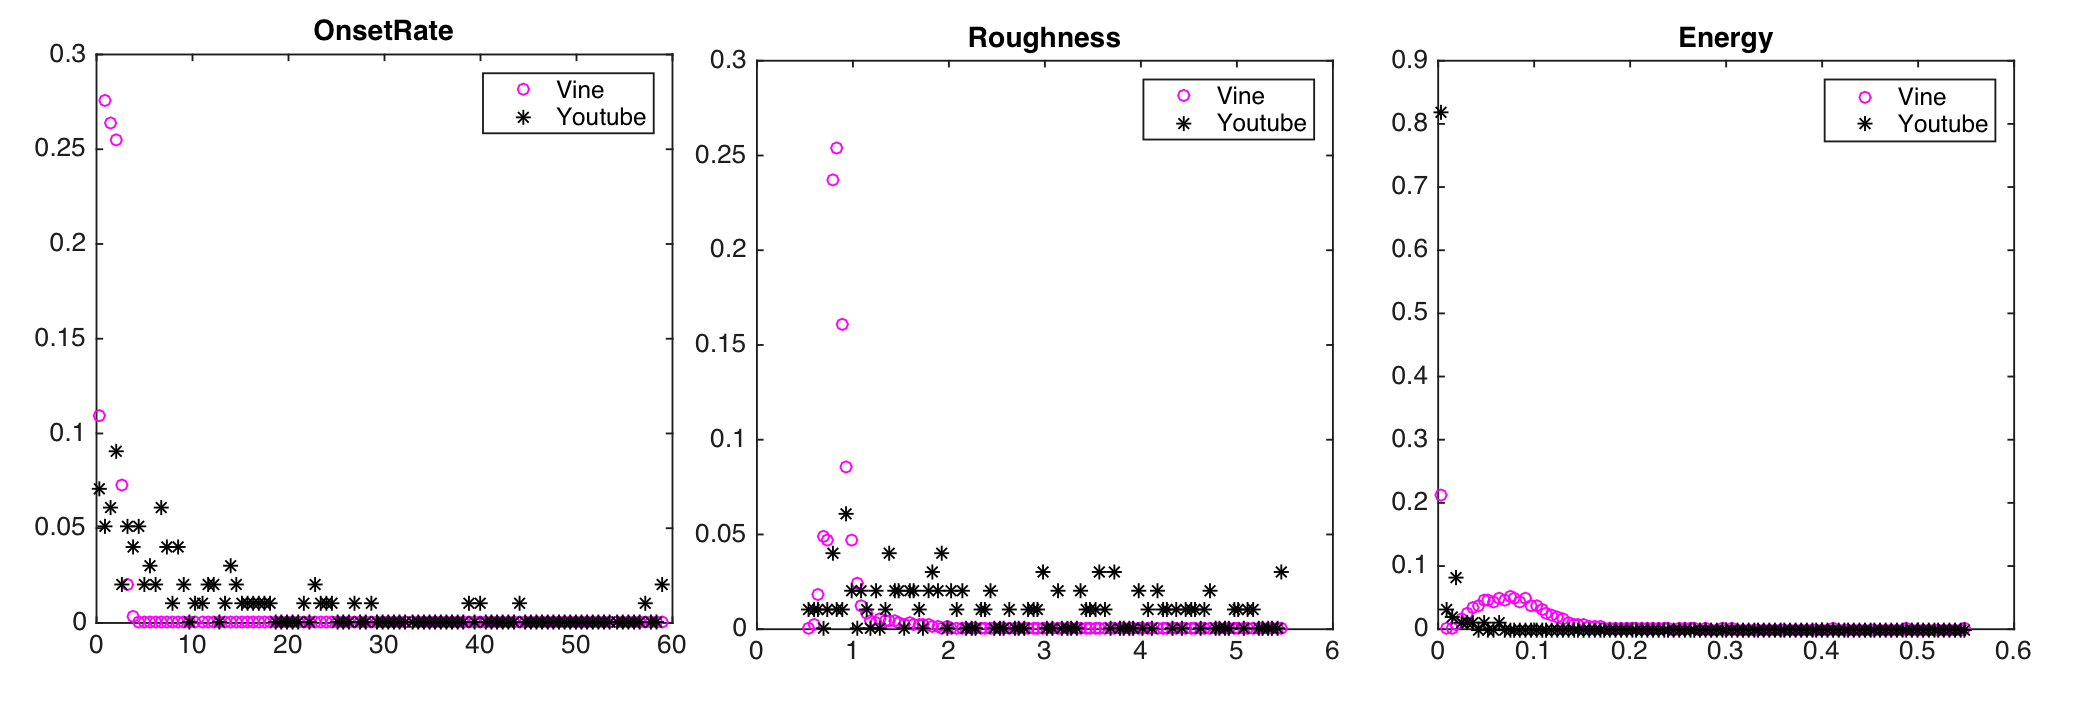
\includegraphics[width=\columnwidth]{plots/comparison/audio}
\caption{\textsl{ Distributions of the most diverging audio features across platforms.}}
\label{fig:comparison_audio}
\end{figure}

\begin{figure}[!htb]
\centering
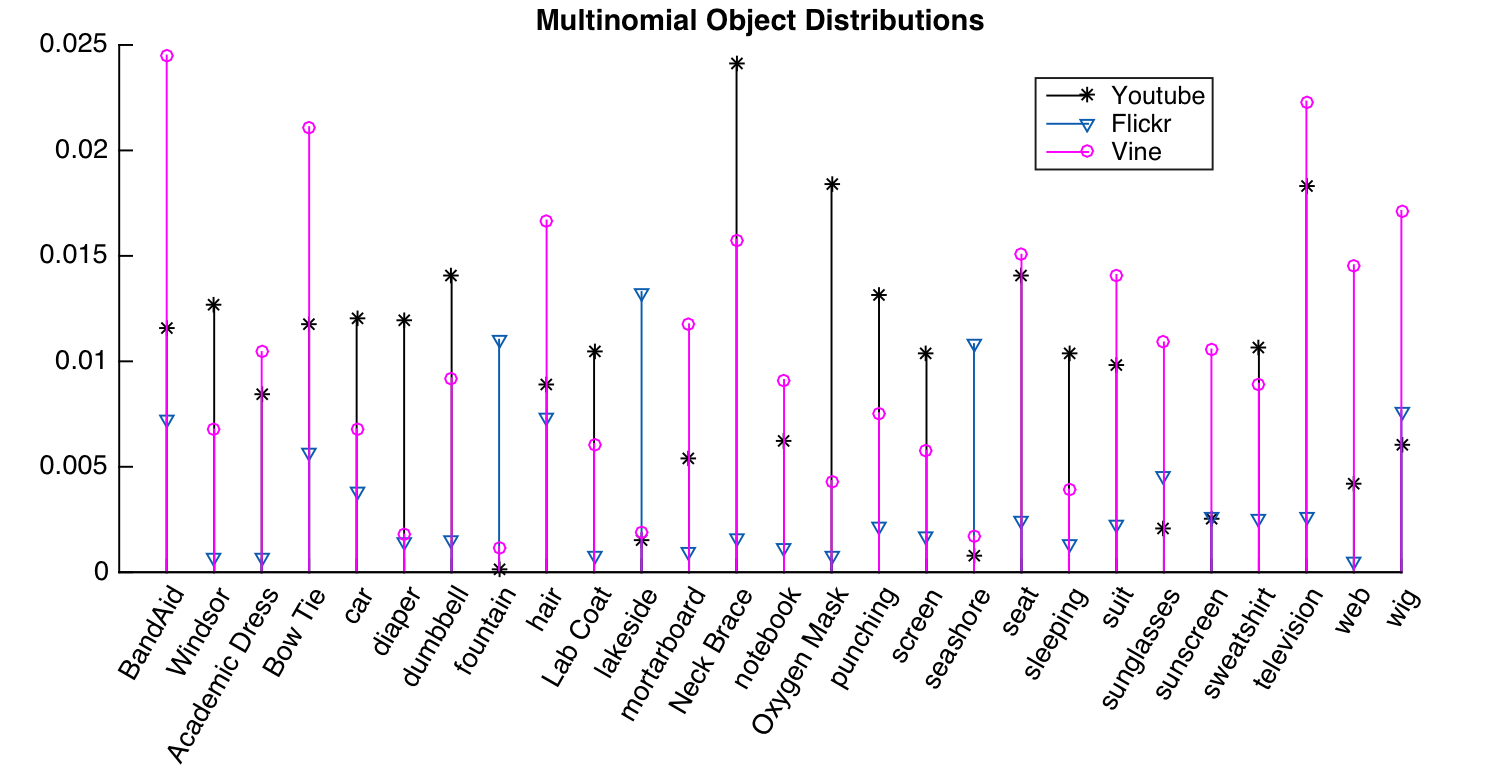
\includegraphics[width=\columnwidth]{plots/comparison/objects}
\caption{\textsl{ Distributions of the most distant object occurrences across platforms, showing a preoccupation with fun and entertainment on Vine, `traditional' popular subjects such as kids, cars and violence on YouTube, and photographic scenery on Flickr.}}
\label{fig:comparison_objects}
\end{figure}

\subsection{Visual Semantics Comparison.} 
Finally, we examine platform differences in terms of the visual objects they focus on.  We use deep learning-based object detectors from ImageNet~\cite{krizhevsky2012imagenet} on each visual item (Flickr images or frame samples from YouTube and Vine videos), and retain the labels of top-5 objects detected. We then aggregate such information at a platform level by computing the multinomial distribution of the detected objects for all Flickr images, Vine videos, and Youtube videos.  Such distributions reflect  the frequency of visual objects in typical popular videos of each platform (e.g. how often does a cat appear in a YouTube video?). Again, we then use symmetric KL divergence to compare object distributions across platforms.



 From Fig.~\ref{fig:comparisontable}, we see that, in the object space, Youtube and Flickr are equally distant from Vine. By looking at element-wise differences across distributions, we then rank objects according to how different their frequencies are for the 3 platforms, and report the top results in Fig.~\ref{fig:comparison_objects}. Vine can be clearly distinguished from the other 2 media due to the higher presence of objects related to celebrations, fun and entertainment (\emph{academic dress} ,\emph{wig}, \emph{tv}, \emph{sunglasses}). Viral Youtube videos prefer popular subjects such as kids (\emph{diaper}), cars, and  violent scenes (\emph{punching}, \emph{neck brace}). Finally, Flickr pictures can be distinguished with the presence of visual concepts typical of photographic sceneries (\emph{lakeside}, \emph{seashore}). These results suggest that the three platforms are used for different purposes, with Vine being more of an immediate medium, `capturing the moment' as it happens. This may help explain the nature of user engagement we observe in the rest of the paper.
%


